% THIS DOCUMENT IS FOLLOWS THE VOLERE TEMPLATE BY Suzanne Robertson and James Robertson
% ONLY THE SECTION HEADINGS ARE PROVIDED
%
% Initial draft from https://github.com/Dieblich/volere
%
% Risks are removed because they are covered by the Hazard Analysis
\documentclass[12pt]{article}

\usepackage{booktabs}
\usepackage{tabularx}
\usepackage{hyperref}
\usepackage{float}
\usepackage{graphicx}
\usepackage{longtable}
\hypersetup{
    bookmarks=true,         % show bookmarks bar?
      colorlinks=true,      % false: boxed links; true: colored links
    linkcolor=red,          % color of internal links (change box color with linkbordercolor)
    citecolor=green,        % color of links to bibliography
    filecolor=magenta,      % color of file links
    urlcolor=cyan           % color of external links
}

\newcommand{\lips}{\textit{Insert your content here.}}

%% Comments

\usepackage{color}

\newif\ifcomments\commentstrue %displays comments
%\newif\ifcomments\commentsfalse %so that comments do not display

\ifcomments
\newcommand{\authornote}[3]{\textcolor{#1}{[#3 ---#2]}}
\newcommand{\todo}[1]{\textcolor{red}{[TODO: #1]}}
\else
\newcommand{\authornote}[3]{}
\newcommand{\todo}[1]{}
\fi

\newcommand{\wss}[1]{\authornote{blue}{SS}{#1}} 
\newcommand{\plt}[1]{\authornote{magenta}{TPLT}{#1}} %For explanation of the template
\newcommand{\an}[1]{\authornote{cyan}{Author}{#1}}

%% Common Parts

\newcommand{\progname}{Software Engineering} % PUT YOUR PROGRAM NAME HERE
\newcommand{\authname}{Team \#11, OKKM Insights
\\ Mathew Petronilho
\\ Oleg Glotov
\\ Kyle McMaster
\\ Kartik Chaudhari} % AUTHOR NAMES                  

\usepackage{hyperref}
    \hypersetup{colorlinks=true, linkcolor=blue, citecolor=blue, filecolor=blue,
                urlcolor=blue, unicode=false}
    \urlstyle{same}
                                


\begin{document}

\title{Software Requirements Specification for \progname: subtitle describing software} 
\author{\authname}
\date{\today}
	
\maketitle

~\newpage

\pagenumbering{roman}

\tableofcontents

~\newpage

\section*{Revision History}

\begin{tabularx}{\textwidth}{p{3cm}p{2cm}X}
\toprule {\textbf{Date}} & {\textbf{Version}} & {\textbf{Notes}}\\
\midrule
Date 1 & 1.0 & Notes\\
Date 2 & 1.1 & Notes\\
\bottomrule
\end{tabularx}

~\\

~\newpage
\section{Purpose of the Project}
\subsection{User Business}
\lips
\subsection{Goals of the Project}
\lips
\section{Stakeholders}
\subsection{Client}
\lips
\subsection{Customer}
\lips
\subsection{Other Stakeholders}
\lips
\subsection{Hands-On Users of the Project}
\lips
\subsection{Personas}
\lips
\subsection{Priorities Assigned to Users}
\lips
\subsection{User Participation}
\lips
\subsection{Maintenance Users and Service Technicians}
\lips

\section{Mandated Constraints}
\subsection{Solution Constraints}
\lips
\subsection{Implementation Environment of the Current System}
\lips
\subsection{Partner or Collaborative Applications}
\lips
\subsection{Off-the-Shelf Software}
\lips
\subsection{Anticipated Workplace Environment}
\lips
\subsection{Schedule Constraints}
\lips
\subsection{Budget Constraints}
\lips
\subsection{Enterprise Constraints}
\lips

\section{Naming Conventions and Terminology}
\subsection{Glossary of All Terms, Including Acronyms, Used by Stakeholders
involved in the Project}
\begin{table}[H]
    \centering
    \begin{tabular}{|p{0.3\linewidth} | p{0.7\linewidth}| }
    \hline
    \textbf{Term} & \textbf{Definition}\\
    \hline
    Labelers & Users of our application that will be labeling photos shown to them for a monetary reward\\
    \hline
    \end{tabular}
    \caption{Naming Conventions and Terminology}
\end{table}

\section{Relevant Facts And Assumptions}
\subsection{Relevant Facts}
\lips
\subsection{Business Rules}
\lips
\subsection{Assumptions}
\lips

\section{The Scope of the Work}
\subsection{The Current Situation}
\lips
\subsection{The Context of the Work}
\lips
\subsection{Work Partitioning}
\lips
\subsection{Specifying a Business Use Case (BUC)}
\lips

\section{Business Data Model and Data Dictionary}
\subsection{Business Data Model}
\lips
\subsection{Data Dictionary}
\lips

\section{The Scope of the Product}
\subsection{Product Boundary}
The use case diagram depicted below identifies the boundaries between the users and the product.
\begin{figure}[H]
    \centering
    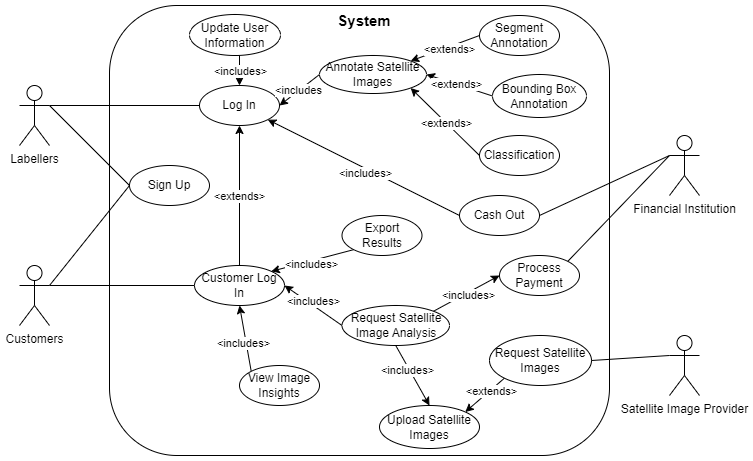
\includegraphics[scale=0.63]{useCaseDiagram.png}
    \caption{Use Case diagram}
    \label{fig:usecase}
\end{figure}
\subsection{Product Use Case Table}
\begin{longtable}
 {p{0.1\textwidth} | p{0.35\textwidth} | p{0.2\textwidth} | p{0.35\textwidth}}
  \toprule
  \textbf{PUC No} & \textbf{PUC Name} & \textbf{Actor/s} & \textbf{Input \& Output}\\
  \midrule
  1 & Sign Up & Labelers, Customers & Personal information \& credentials (in), New account (out)\\
  \midrule
  2 & Log In & Labelers & Credentials (in)\\
  \midrule
  3 & Customer Log In & Customers & Credentials (in)\\
  \midrule
  4 & Update User Information & Labelers, Customers & Information to change (in),  Updated information (out)\\
   \midrule
  5 & Annotate Images & Labelers & Image \& annotation (in), Labeled image (out)\\
  \midrule
  6 & Segment Annotation & Labelers & Segmented image \& user selections (in), Image with labeled segments (out)\\
  \midrule
  7 & Bounding Box Annotation & Labelers & Image \& box annotations (in), Image with labeled boxes (out)\\
  \midrule
  8 & Classification & Labelers & Image \& choices (in), Image labeled with the selected choice (out)\\
  \midrule
   9 & Cash Out & Labelers, Financial Institution & Financial information (in), Payment to user (out)\\
  \midrule
  10 & View Image Insights & Customers & Request to view insights (in), Image insights (out)\\
  \midrule
  11 & Export Results & Customers & Request to export results (in), Results in downloadable format (out)\\
  \midrule
  12 & Request Image Analysis & Customers & Labels, images \& examples (in) \\
  \midrule
  13 & Upload Images & Customers & Images (in)\\
  \midrule
  14 & Request Images & Customers, Satellite Image Provider & Description of images wanted (in), Images (out)\\
  \midrule
  15 & Process Payment & Customers, Financial Institution & Financial information (in), Payment to app (out)\\
  \bottomrule
  \caption{Product Use Cases} \label{TblPUC}\\
\end{longtable}
\subsection{Individual Product Use Cases (PUC's)}
\subsubsection{PUC 1 - Sign Up}
\textbf{Primary Actors:} Labelers, Customers\\ 
\textbf{Precondition:} None\\
\textbf{Trigger:} User selects create an account\\
\textbf{Success Scenario:}
\begin{enumerate}
    \item User provides the required information and agrees with the privacy policy of the application
    \item System verifies all required information has been provided and is of valid syntax
    \item System securely registers the given information
    \item User is directed to the login page
\end{enumerate}
\textbf{Post-condition:} User has successfully created an account and the application has securely stored their information

\subsubsection{PUC 2 - Log In}
\textbf{Primary Actors:} Labelers\\ 
\textbf{Precondition:} Labeler has signed up for an account\\
\textbf{Trigger:} Labeler selects log in\\
\textbf{Success Scenario:}
\begin{enumerate}
    \item Labeler enters credentials
    \item System verifies all required information has been provided and matches the stored records
    \item Labeler is redirected to the home page as a logged-in user
\end{enumerate}
\textbf{Post-condition:} The labeler has access to their account. All account related information, such as labeling progress, is accurately represented

\subsubsection{PUC 3 - Customer Log In}
\textbf{Primary Actors:} Customers\\ 
\textbf{Precondition:} Customer has signed up for an account\\
\textbf{Trigger:} Customer selects log in\\
\textbf{Success Scenario:}
\begin{enumerate}
    \item Customer enters credentials
    \item System verifies all required information has been provided and matches the stored records
    \item Customer is redirected to the home page as a logged-in customer, which gives them access to more features than a labeler
\end{enumerate}
\textbf{Post-condition:} The customer has access to their account and all their current image analysis projects

\subsubsection{PUC 4 - Update User Information}
\textbf{Primary Actors:} Labelers, Customers\\ 
\textbf{Precondition:} User has logged in\\
\textbf{Trigger:} User selects update information\\
\textbf{Success Scenario:}
\begin{enumerate}
    \item User enters updated information
    \item System verifies the new information has valid syntax
    \item System updates the information
    \item User is given a confirmation that their information has been updated
\end{enumerate}
\textbf{Post-condition:} The information that the system stores about the user has been updated

\subsubsection{PUC 5 - Annotate Satellite Images}
\textbf{Primary Actors:} Labelers\\ 
\textbf{Precondition:} Labeler has logged in\\
\textbf{Trigger:} Labeler selects a listed project\\
\textbf{Success Scenario:}
\begin{enumerate}
    \item A satellite image related to the selected project and a description of what to annotate is shown to the labeler
    \item The labeler annotates the satellite image to the best of their ability
    \item The annotated satellite image is submitted by the labeler
    \item The labeler is rewarded and the satellite image is stored by the system
    \item If the labeler skips the image rather than submits it, then the annotated image will not be stored by the system and the labeler will not receive a reward
    \item The next satellite image of the selected project is shown to the labeler and the process repeats
\end{enumerate}
\textbf{Post-condition:} All submitted annotated satellite images are stored by the system. The labeler's reward balance is updated to reflect their submissions

\subsubsection{PUC 6 - Segment Annotation}
\textbf{Primary Actors:} Labelers\\ 
\textbf{Precondition:} Labeler has logged in\\
\textbf{Trigger:} Labeler selects a listed project\\
\textbf{Success Scenario:}
\begin{enumerate}
    \item The same as Annotate Images, but the labeler is given a satellite image segmented into different parts and must label each segment to the best of their ability 
\end{enumerate}
\textbf{Post-condition:} All submitted annotated satellite images are stored by the system. The labeler's reward balance is updated to reflect their submissions

\subsubsection{PUC 7 - Bounding Box Annotation}
\textbf{Primary Actors:} Labelers\\ 
\textbf{Precondition:} Labeler has logged in\\
\textbf{Trigger:} Labeler selects a listed project\\
\textbf{Success Scenario:}
\begin{enumerate}
    \item The same as Annotate Images, but the labeler must annotate areas of the satellite image by drawing boxes and providing a label for each box
\end{enumerate}
\textbf{Post-condition:} All submitted annotated satellite images are stored by the system. The labeler's reward balance is updated to reflect their submissions

\subsubsection{PUC 8 - Classification}
\textbf{Primary Actors:} Labelers\\ 
\textbf{Precondition:} Labeler has logged in\\
\textbf{Trigger:} Labeler selects a listed project\\
\textbf{Success Scenario:}
\begin{enumerate}
    \item The same as Annotate Images, but the labeler must classify what category an satellite image belongs to given several options
\end{enumerate}
\textbf{Post-condition:} All submitted annotated satellite images are stored by the system. The labeler's reward balance is updated to reflect their submissions

\subsubsection{PUC 9 - Cash Out}
\textbf{Primary Actors:} Labelers\\
\textbf{Secondary Actor:} Financial Institution\\
\textbf{Precondition:} Labeler has logged in and their reward balance is at least \$1\\
\textbf{Trigger:} Labeler selects cash out\\
\textbf{Success Scenario:}
\begin{enumerate}
    \item The system retrieves the labeler's payment information
    \item The labeler confirms it is correct, or updates their information accordingly
    \item The system sends a payment to the labeler through their financial institution
    \item The labeler's reward balance is set back to \$0
\end{enumerate}
\textbf{Post-condition:} The financial account that the labeler provided has gained money equal to the labeler's reward balance

\subsubsection{PUC 10 - View Image Insights}
\textbf{Primary Actors:} Customers\\
\textbf{Precondition:} Customer has logged in and has at least one satellite image analysis project\\
\textbf{Trigger:} Customer selects insights for a project\\
\textbf{Success Scenario:}
\begin{enumerate}
    \item The system provides the customer with a progress update, key statistics, and an overview of current labels for specific satellite images
    \item The customer selects a specific image to view insights 
    \item The system gets the information it has stored related to the image and provides insights such as confidence level of annotations
\end{enumerate}
\textbf{Post-condition:} The customer has knowledge about how their project is progressing and if the labeling of the satellite images has been complete

\subsubsection{PUC 11 - Export Results}
\textbf{Primary Actors:} Customers\\
\textbf{Precondition:} Customer has logged in, has at least one satellite image analysis project, and all labeled satellite images in that project have an acceptable accuracy\\
\textbf{Trigger:} Customer selects export data\\
\textbf{Success Scenario:}
\begin{enumerate}
    \item The system retrieves all the labeled satellite images associated with the project
    \item The system asks the customer where they would like the images to be saved
    \item The customer specifies the save location
    \item The images are downloaded to the specified location
\end{enumerate}
\textbf{Post-condition:} The customer has complete access to the labeled dataset of satellite images

\subsubsection{PUC 12 - Request Image Analysis}
\textbf{Primary Actors:} Customers\\
\textbf{Precondition:} Customer has logged in\\
\textbf{Trigger:} Customer creates a new project request\\
\textbf{Success Scenario:}
\begin{enumerate}
    \item The system prompts the customer with a form to fill out regarding information about the project such as what is to be labeled
    \item The customer fills out the form and submits it
    \item The system confirms the forms information is valid. It prompts the customer to upload the satellite image dataset to be analyzed
    \item The customer uploads their own satellite images or requests the system to get images for them
    \item The system asks the customer to provide sample labeled images that can be shared with labelers
    \item The customer uploads sample labeled images
    \item Based on the size and difficulty of the project, the system provides the total cost of the project to the customer
    \item The customer provides their payment details
    \item The system processes the payment
    \item The system makes the project available to labelers so they can annotate the satellite images
\end{enumerate}
\textbf{Post-condition:} The image analysis project has been created and labelers can start annotating the satellite images

\subsubsection{PUC 13 - Upload Satellite Images}
\textbf{Primary Actors:} Customers\\
\textbf{Precondition:} Customer has logged in and has created a new project request\\
\textbf{Trigger:} Customer submits the information form for a new project\\
\textbf{Success Scenario:}
\begin{enumerate}
    \item The system prompts the customer to upload the images they would like to be analyzed
    \item The customer selects the images they want analyzed and uploads them
    \item The system stores the images with a reference to the project
\end{enumerate}
\textbf{Post-condition:} The system has all the images that will be analyzed for the project

\subsubsection{PUC 14 - Request Satellite Images}
\textbf{Primary Actors:} Customers\\
\textbf{Secondary Actors:} Satellite Image Provider\\
\textbf{Precondition:} Customer has logged in and has created a new project request\\
\textbf{Trigger:} Customer submits the information form for a new project\\
\textbf{Success Scenario:}
\begin{enumerate}
    \item The system prompts the customer about the type of satellite images they want. This could be satellite images from a specific time frame in a specific area
    \item The customer specifies the type of satellite images they want for analysis
    \item The system contacts a satellite image provider, and pays a fee to them in exchange for the images. The fee is charged to the customer
    \item The system stores the images with a reference to the project
\end{enumerate}
\textbf{Post-condition:} The system has all the satellite images that will be analyzed for the project

\subsubsection{PUC 15 - Process Payment}
\textbf{Primary Actors:} Customers\\
\textbf{Secondary Actor:} Financial Institution\\
\textbf{Precondition:} Customer has logged in and has created a new project request\\
\textbf{Trigger:} Customer has filled out all the details of the project and uploaded all the photos\\
\textbf{Success Scenario:}
\begin{enumerate}
    \item The system retrieves the customer's payment information
    \item The customer confirms it is correct, or updates their information accordingly
    \item The system sends a payment request to the customer's financial institution
    \item The financial institution validates the payment information and sends the payment
    \item The payment is deposited in the financial account associated with the system
\end{enumerate}
\textbf{Post-condition:} The fees for facilitating the project have been paid

\section{Functional Requirements}
\subsection{Functional Requirements}
\lips

\section{Look and Feel Requirements}
\subsection{Appearance Requirements}
\lips
\subsection{Style Requirements}
\lips

\section{Usability and Humanity Requirements}
\subsection{Ease of Use Requirements}
\lips
\subsection{Personalization and Internationalization Requirements}
\lips
\subsection{Learning Requirements}
\lips
\subsection{Understandability and Politeness Requirements}
\lips
\subsection{Accessibility Requirements}
\lips

\section{Performance Requirements}
\subsection{Speed and Latency Requirements}
\lips
\subsection{Safety-Critical Requirements}
\lips
\subsection{Precision or Accuracy Requirements}
\lips
\subsection{Robustness or Fault-Tolerance Requirements}
\lips
\subsection{Capacity Requirements}
\lips
\subsection{Scalability or Extensibility Requirements}
\lips
\subsection{Longevity Requirements}
\lips

\section{Operational and Environmental Requirements}
\subsection{Expected Physical Environment}
\lips
\subsection{Wider Environment Requirements}
\lips
\subsection{Requirements for Interfacing with Adjacent Systems}
\lips
\subsection{Productization Requirements}
\lips
\subsection{Release Requirements}
\lips

\section{Maintainability and Support Requirements}
\subsection{Maintenance Requirements}
\lips
\subsection{Supportability Requirements}
\lips
\subsection{Adaptability Requirements}
\lips

\section{Security Requirements}
\subsection{Access Requirements}
\lips
\subsection{Integrity Requirements}
\lips
\subsection{Privacy Requirements}
\lips
\subsection{Audit Requirements}
\lips
\subsection{Immunity Requirements}
\lips

\section{Cultural Requirements}
\subsection{Cultural Requirements}
\lips

\section{Compliance Requirements}
\subsection{Legal Requirements}
\lips
\subsection{Standards Compliance Requirements}
\lips

\section{Open Issues}
\lips

\section{Off-the-Shelf Solutions}
\subsection{Ready-Made Products}
\lips
\subsection{Reusable Components}
\lips
\subsection{Products That Can Be Copied}
\lips

\section{New Problems}
\subsection{Effects on the Current Environment}
\lips
\subsection{Effects on the Installed Systems}
\lips
\subsection{Potential User Problems}
\lips
\subsection{Limitations in the Anticipated Implementation Environment That May
Inhibit the New Product}
\lips
\subsection{Follow-Up Problems}
\lips

\section{Tasks}
\subsection{Project Planning}
\lips
\subsection{Planning of the Development Phases}
\lips

\section{Migration to the New Product}
\subsection{Requirements for Migration to the New Product}
\lips
\subsection{Data That Has to be Modified or Translated for the New System}
\lips

\section{Costs}
\lips
\section{User Documentation and Training}
\subsection{User Documentation Requirements}
\lips
\subsection{Training Requirements}
\lips

\section{Waiting Room}
\lips

\section{Ideas for Solution}
\lips

\newpage{}
\section*{Appendix --- Reflection}

The information in this section will be used to evaluate the team members on the
graduate attribute of Lifelong Learning.  Please answer the following questions:

\begin{enumerate}
  \item What knowledge and skills will the team collectively need to acquire to
  successfully complete this capstone project?  Examples of possible knowledge
  to acquire include domain specific knowledge from the domain of your
  application, or software engineering knowledge, mechatronics knowledge or
  computer science knowledge.  Skills may be related to technology, or writing,
  or presentation, or team management, etc.  You should look to identify at
  least one item for each team member.
  \item For each of the knowledge areas and skills identified in the previous
  question, what are at least two approaches to acquiring the knowledge or
  mastering the skill?  Of the identified approaches, which will each team
  member pursue, and why did they make this choice?
\end{enumerate}

\end{document}
